\documentclass[border=10pt]{standalone}

\usepackage{tikz}
\usepackage{tikzsymbols}
\usetikzlibrary{calc,patterns,shapes.geometric}

\def\centerarc[#1](#2)(#3:#4:#5){\draw[#1] ($(#2)+({#5*cos(#3)},{#5*sin(#3)})$) arc (#3:#4:#5);}

\begin{document}
	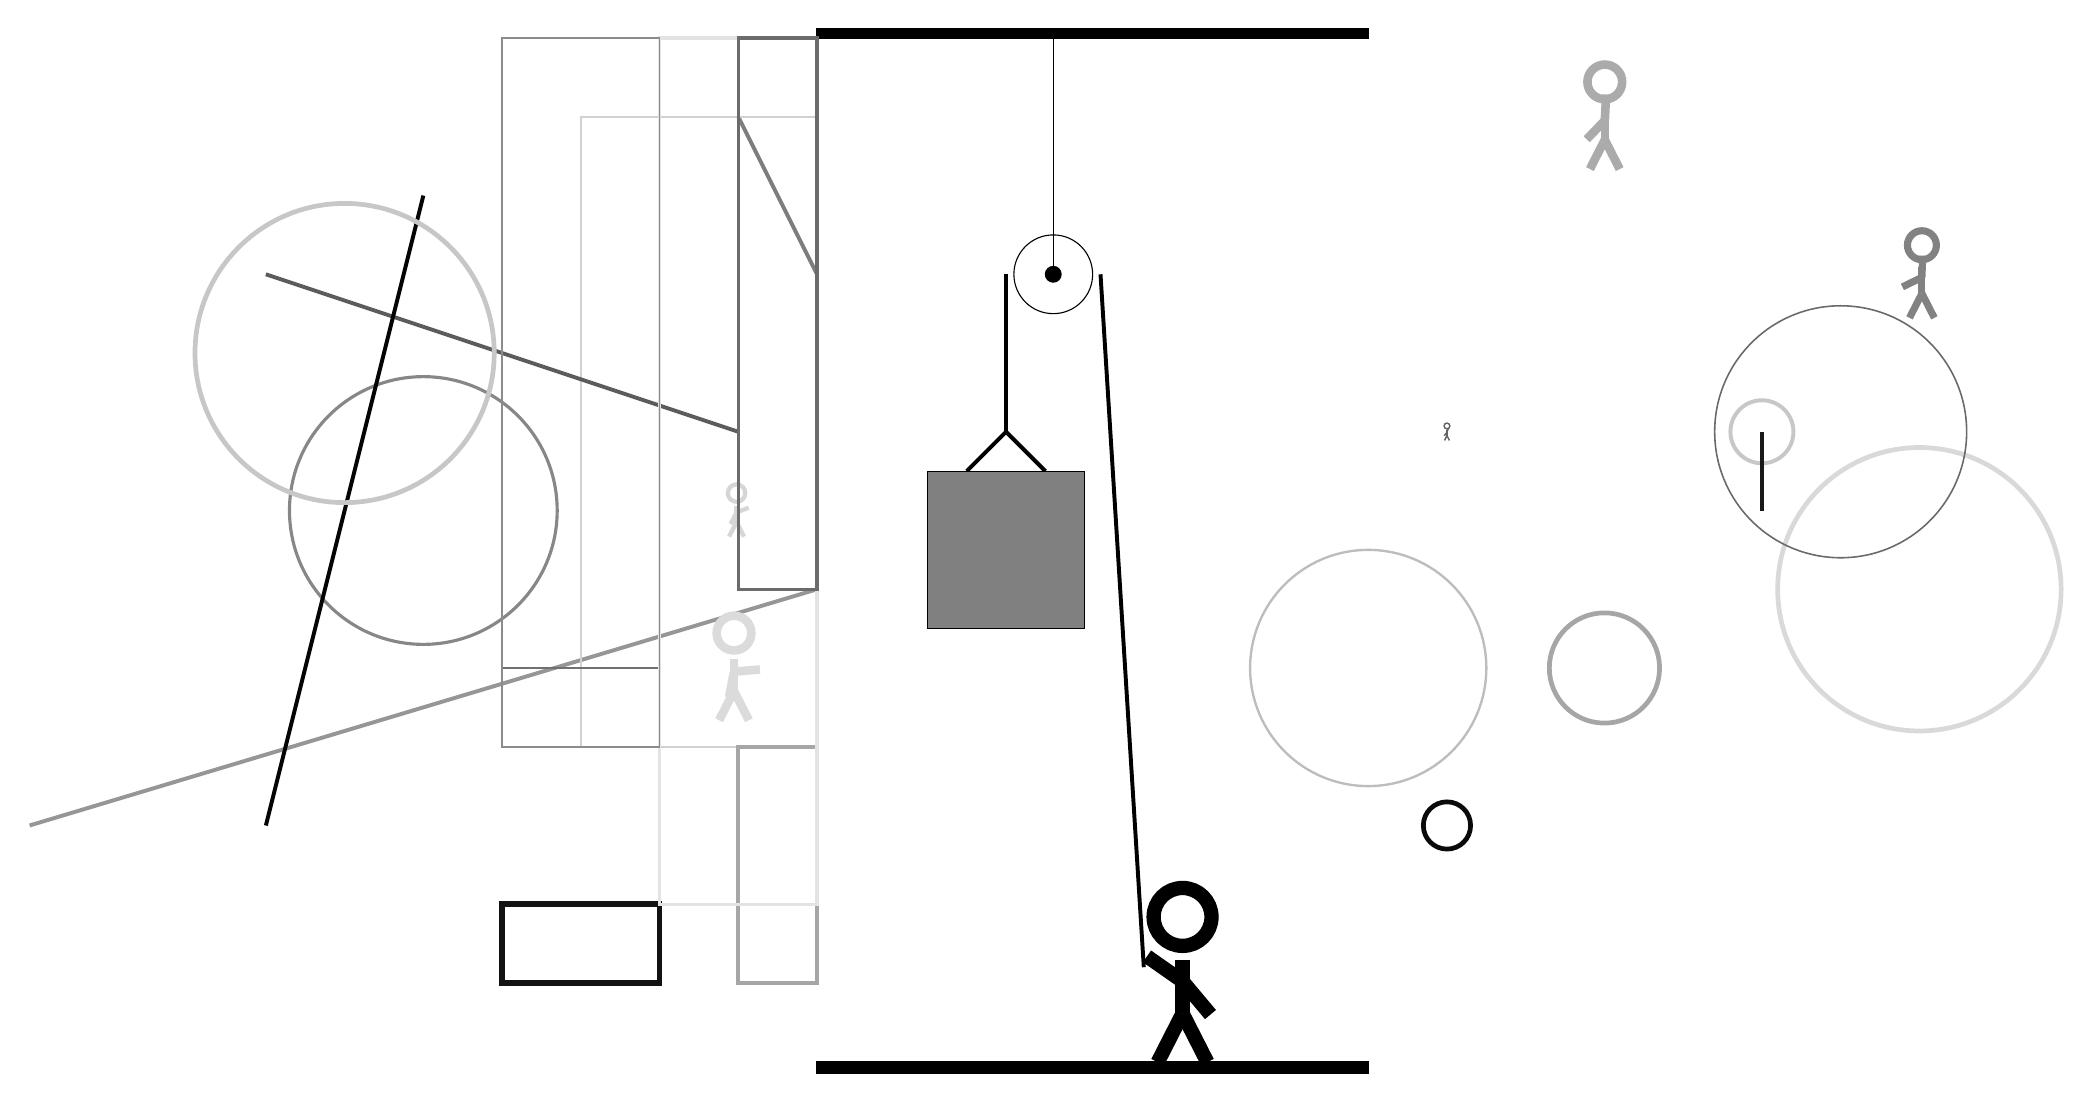
\begin{tikzpicture}
		%%%%% START %%%%%
		
		\draw[fill=black] (-2, 10) rectangle (5, 10.125);
		
		\draw (1, 7) circle (0.5);
		\draw[fill=black] (1, 7) circle (0.1);
		\draw (1, 10) -- (1, 7);
		
		\draw[line width=0.5mm] (-0.1, 4.5) -- (0.4, 5.0) -- (0.9, 4.5);
		\draw[fill=black!50] (-0.6, 4.5) rectangle (1.4, 2.5);
		
		\draw[line width=0.5mm] (0.4, 7) -- (0.4, 5.0);
		\centerarc[line width=0.5mm](1, 7)(0:180:0.6);
		\draw[line width=0.5mm](1.6, 7) -- (2.15, -1.8);
		
		\draw [line width=0.5mm, color=black!22](10, 5) circle (0.4);
		
		\draw [line width=0.4mm, color=black!35](-8, -1) circle (0.0);
		\node[line width=0.5mm, color=black!16] at (-3, 4) {\Strichmaxerl[3][63][21]};
		\draw[line width=0.7mm, color=black!93] (-4, -1) rectangle (-6, -2);
		\draw [line width=0.6mm, color=black!15](12, 3) circle (1.8);
		\draw [line width=0.4mm, color=black!47](-7, 4) circle (1.7);
		\node[line width=0.3mm, color=black!62] at (6, 5) {\Strichmaxerl[1][50][71]};
		\draw[line width=0.5mm, color=black!41](-2, 3) -- (-12, 0);
		\draw[line width=0.5mm, color=black!51](-2, 7) -- (-3, 9);
		\draw[line width=0.2mm, color=black!18] (-2, 9) rectangle (-5, 1);
		
		\draw [line width=0.6mm, color=black!96](6, 0) circle (0.3);
		\node[line width=0.7mm, color=black!33] at (8, 9) {\Strichmaxerl[6][46][87]};
		\draw[line width=0.5mm, color=black!64](-3, 5) -- (-9, 7);
		
		\node[line width=0.7mm, color=black!49] at (12, 7) {\Strichmaxerl[5][26][88]};
		\draw[line width=0.5mm, color=black!98](-7, 8) -- (-9, 0);
		\draw [line width=0.3mm, color=black!26](5, 2) circle (1.5);
		\draw[line width=0.3mm, color=black!56] (-4, 10) rectangle (-6, 2);
		\draw[line width=0.5mm, color=black!35] (-2, 1) rectangle (-3, -2);
		\draw[line width=0.5mm, color=black!90](10, 4) -- (10, 5);
		\draw [line width=0.6mm, color=black!22](-8, 6) circle (1.9);
		\draw[line width=0.4mm, color=black!11] (-4, -1) rectangle (-2, 10);
		\draw [line width=0.6mm, color=black!35](8, 2) circle (0.7);
		\draw[line width=0.2mm, color=black!45] (-4, 1) rectangle (-6, 10);
		\draw[line width=0.4mm, color=black!58] (-2, 10) rectangle (-3, 3);
		\draw [line width=0.2mm, color=black!59](11, 5) circle (1.6);
		\node[line width=0.5mm, color=black!14] at (-3, 2) {\Strichmaxerl[6][79][5]};
		
		
		\node at (2.6, -1.9) {\Strichmaxerl[10][-35][-50]};
		
		\draw[fill=black] (-2, -3) rectangle (5, -3.15);
		
		%%%%% END %%%%%
	\end{tikzpicture}
\end{document}